
Il teorema di Kutta--Jukowski lega la circolazione attorno a un corpo alla portanza generata, nelle ipotesi di correnti incomprimibili, non viscose, irrotazionali.
Utilizzando i bilanci integrali di massa e di quantità di moto, ricaveremo il teorema di Kutta--Jukowski per un problema bidimensionale stazionario.
Utilizziamo un sistema di coordinate cartesiano, con l'asse $x$ orientato come la velocità asintotica $\bm{U}_{\infty} = U_{\infty} \bm{\hat{x}}$ che investe il corpo. Scriviamo poi il campo di velocità come la somma della velocità asintotica e una velocità \textit{di preturbazione} $\bm{u}'(\bm{r})$,
\begin{equation}\label{eqn:vel:dec}
 \bm{u}(\bm{r}) = \bm{U}_{\infty} + \bm{u}'(\bm{r}) \ .
\end{equation}
L'unico ``atto di fede'' che vi viene richiesto riguarda l'andamento asintotico della velocità di perturbazione all'infinito. Si può dimostrare che la velocità di perturbazione è proporzionale all'inverso della distanza dal corpo,
\begin{equation}
 |\bm{u}'(\bm{r})| \sim \dfrac{1}{|\bm{r}|} \quad, \qquad |\bm{r}| \rightarrow \infty \ .
\end{equation}
Utilizzando il bilancio integrale di quantità di moto per il volume di controllo euleriano $V$ rappresentato in figura {\color{red} \dots}, si può valurare la forza esercitata dal fluido sul corpo,
\begin{equation}
 \bm{R} = - \oint_S \rho \bm{u} \bm{u} \cdot \bm{\hat{n}} - \oint_S P \bm{\hat{n}} \ ,
\end{equation}
Nell'ipotesi che la corrente sia irrotazionale, si può utilizzare il teorema di Bernoulli per valutare il campo di pressione in funzione della velocità e delle condizioni asintotiche,
\begin{equation}
 P = P_{\infty} + \dfrac{1}{2} \rho U_{\infty}^2 - \dfrac{1}{2} \rho |\bm{u}|^2 \ ,
\end{equation}
e riscrivere l'espressione della forza agente sul corpo come,
\begin{equation}
 \bm{R} = - \oint_S \rho \bm{u} \bm{u} \cdot \bm{\hat{n}} + \oint_S \dfrac{1}{2} \rho |\bm{u}|^2 \bm{\hat{n}} \ ,
\end{equation}
avendo semplificato gli integrali nulli su una superficie chiusa di una quantità costante moltiplicata per il versore normale.

\begin{figure}[h!]
\centering
 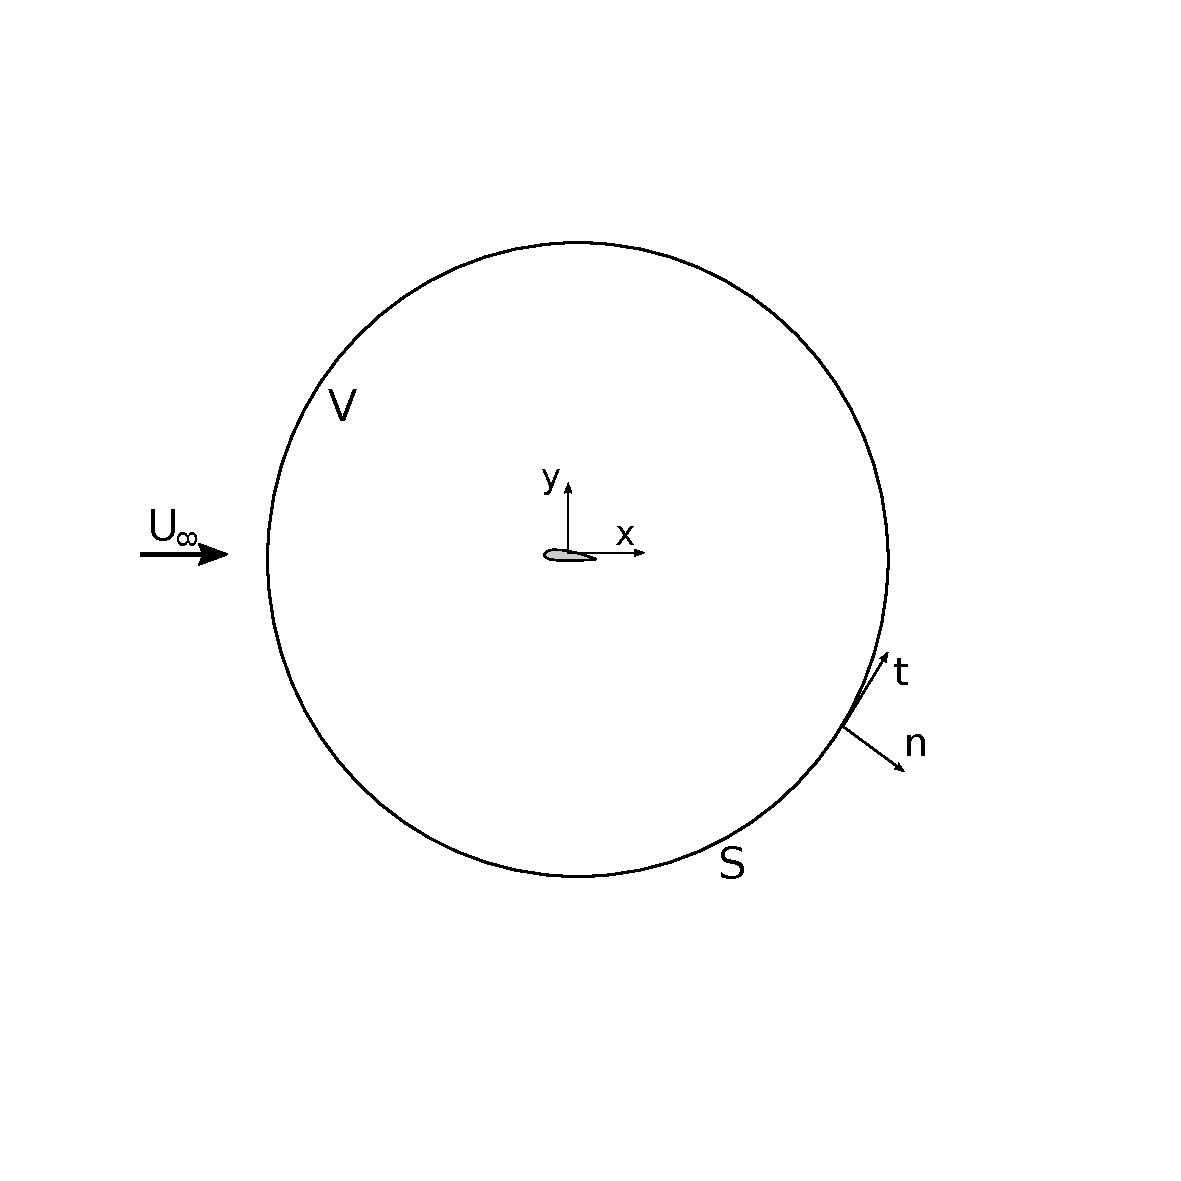
\includegraphics[width=0.75\textwidth, trim= 40 100 100 100, clip]{./fig/kj}
\caption{volume di controllo per la dimostrazione del teorema di Kutta--Jukowski.}\label{fig:kj}
\end{figure}

A questo punto, si può utilizzare l'espressione della velocità (\ref{eqn:vel:dec}), per manipolare gli integrali,
\begin{equation}\label{eqn:kj:1}
\begin{aligned}
 \bm{R} & = - \oint_S \rho \bm{U}_{\infty} \bm{u} \cdot \bm{\hat{n}}
            - \oint_S \rho \bm{u}'         \bm{u} \cdot \bm{\hat{n}} \\
   & \qquad + \oint_S \dfrac{1}{2} \rho U^2_{\infty}  \bm{\hat{n}}
            + \oint_S \rho \bm{U}_{\infty} \cdot \bm{u}' \bm{\hat{n}}
            + \oint_S \rho |\bm{u}'|^2 \bm{\hat{n}} \ .
\end{aligned}
\end{equation}
Il primo integrale è nullo per il bilancio integrale della massa, poiché
\begin{equation}
  \oint_S \rho \bm{U}_{\infty} \bm{u} \cdot \bm{\hat{n}} = 
  \rho \bm{U}_{\infty} \oint_S \bm{u} \cdot \bm{\hat{n}} = 0 \ ,
\end{equation}
se il corpo non inietta fluido nel dominio. Il terzo integrale è nullo.
Il secondo integrale può essere riscritto come
\begin{equation}
- \oint_S \rho \bm{u}'         \bm{u} \cdot \bm{\hat{n}} = 
- \oint_S \rho \bm{u}' \bm{U}_{\infty}\cdot \bm{\hat{n}} 
- \oint_S \rho \bm{u}' \bm{u}'        \cdot \bm{\hat{n}} \ .
\end{equation}
Quando si fa tendere la superficie $S$ all'infinito, la dimensione del dominio di integrazione tende all'infinito come $r$. Poiché $|\bm{u}'| \sim 1/r$ quando $r \rightarrow \infty$, gli integrali quadratici in $\bm{u}'$ tendono a zero.

Rimettendo insieme tutti i pezzi dell'equazione (\ref{eqn:kj:1}), quando $r \rightarrow \infty$, si ottiene
\begin{equation}
 \bm{R} = - \oint_S \rho \bm{u}' \bm{U}_{\infty}\cdot \bm{\hat{n}} 
          + \oint_S \rho \bm{U}_{\infty} \cdot \bm{u}' \bm{\hat{n}} \ .
\end{equation}
Questa espressione può essere manipolata utilizzando l'identità vettoriale $\bm{a} \times (\bm{b} \times \bm{c} ) = (\bm{a} \cdot \bm{c}) \bm{b} - (\bm{a} \cdot \bm{b}) \bm{c}$, per scrivere
\begin{equation}
 \bm{R} = - \rho \bm{U}_\infty \times \oint_S \bm{u}' \times \bm{\hat{n}} \ .
\end{equation}
In due dimensioni, il versore normale alla superficie può essere espresso in funzione del versore tangente,
\begin{equation}
 n_x = t_y \quad , \quad n_y = - t_x \ ,
\end{equation}
e quindi è possibile riscrivere il prodotto vettore $\bm{u}' \times \bm{\hat{n}} = -\bm{\hat{z}} \,(\bm{u}' \cdot \bm{\hat{t}})$, e la risultante sul corpo
\begin{equation}
 \bm{R} = \rho \bm{U}_\infty \times \bm{\hat{z}} \, \oint_S \bm{u}' \cdot \bm{\hat{t}} \ .
\end{equation}
Si può sommare all'integrale il termine nullo $\oint_S \bm{U}_{\infty} \cdot \bm{\hat{t}}$ per ottenere\begin{equation}
 \bm{R} = \rho \bm{U}_\infty \times \bm{\hat{z}} \, \oint_S \bm{u} \cdot \bm{\hat{t}} \ ,
\end{equation}
svolgere il prodotto vettoriale $\bm{U}_{\infty} \times \bm{\hat{z}} = - U_{\infty} \bm{\hat{y}}$, e riconoscere la definizione della circolazione attorno al corpo,
\begin{equation}
 \Gamma = \oint_S \bm{u} \cdot \bm{\hat{t}} \ ,
\end{equation}
per ricavare l'espressione del teorema di Kutta--Jukowski,
\begin{equation}
 \bm{R} = -\rho U_{\infty} \Gamma \bm{\hat{y}} \ .
\end{equation}



